\begin{frame}\frametitle{}

\vspace*{0.2in}

\hspace*{0.0in}\textrm{{\huge\bfseries\color{myOrange} Fr@CEESD}}

\vspace*{0.2in}
\hrule
\begin{center}
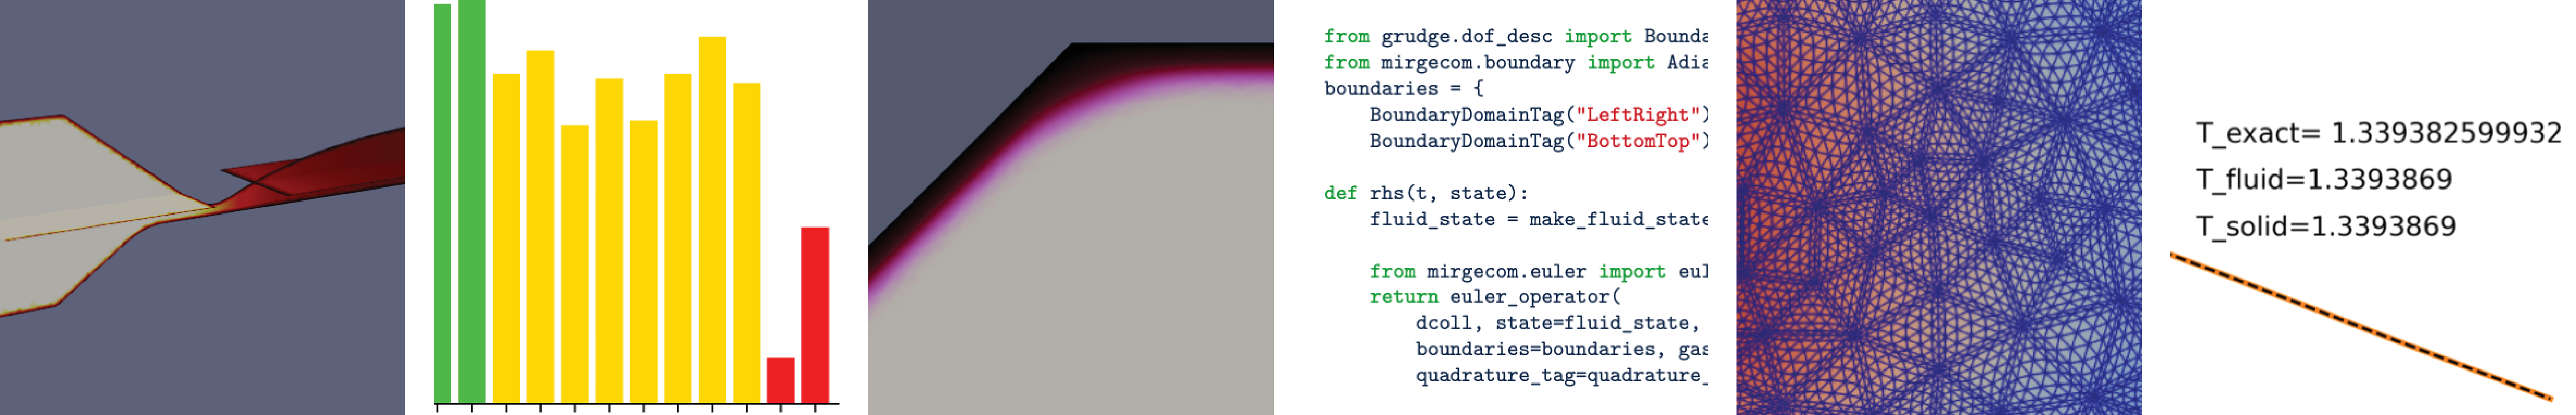
\includegraphics[width=0.7\textwidth]{Figures/coverart-sim.pdf}
\end{center}
\hrule

\vspace*{0.1in}
\hfill\cPI{Mike Campbell} \rPI{(CS)}  % \\
%\ \hbox{}\hfill\cPI{Matt Smith} \rPI{(NCSA)}\\
%\ \hbox{}\hfill\cPI{Mike Campbell} \rPI{(NCSA)}\\
%\ \hbox{}\hfill\cPI{Mike Anderson} \rPI{(NCSA)}

\end{frame}
\begin{frame}{Outline}
\begin{itemize}
    \item \textbf{MIRGE-Com in Y3}
    \begin{itemize}
        \item Architecture Overview
        \item Supported Physics \& Predictive Capabilities
    \end{itemize}
    
    \item \textbf{Scalability Fundamentals}
    \begin{itemize}
        \item Strong Scaling: Speed with Resources
        \item Weak Scaling: Tackling Bigger Problems
        \item Versatility: Dynamic Simulation Adjustments
    \end{itemize}
    
    \item \textbf{MIRGE-Com Scaling in Y3}
    \begin{itemize}
        \item Performance Snapshots
        \begin{itemize}
            \item Weak Scaling Achievements
            \item Strong Scaling Insights
            \item Lassen Monitoring Highlights
        \end{itemize}
        \item Scaling Challenges
        \begin{itemize}
            \item Partitioning \& DAG Splat Issues
            \item Mesh Processing Complexities
            \item DAG Feature Dynamics \& Performance
            \item Upcoming Threats \& Concerns
        \end{itemize}
    \end{itemize}
    
    \item \textbf{Conclusion \& Future Directions}
    \begin{itemize}
        \item Upcoming Review Priorities
        \item Vision \& Long-Term Goals
    \end{itemize}
\end{itemize}
\end{frame}

\begin{frame}
    \centering
    \Large
    \textbf{Diving into MIRGE-Com in Y3}
\end{frame}

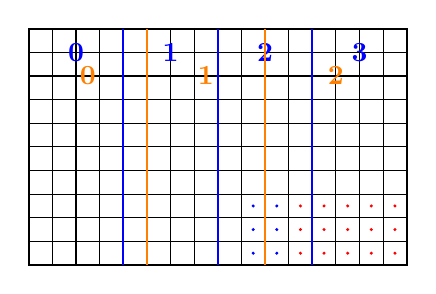
\begin{tikzpicture}[scale=0.3]
    % Grid
    \draw[step=1, thin, black] (0,0) grid (16,10);
    \draw[thick] (0,0) rectangle (16,10);
    
    % Red subregion
    \foreach \i in {11, 12, 13, 14, 15} {
        \foreach \j in {0, 1, 2} {
            \fill[red] (\i+0.5, \j+0.5) circle (2pt);
        }
    }
    
    % Blue subregion
    \foreach \i in {9, 10} {
        \foreach \j in {0, 1, 2} {
            \fill[blue] (\i+0.5, \j+0.5) circle (2pt);
        }
    }

    % Partition lines and labels for 4 partitions (in blue)
    \draw[thick, blue] (4,0) -- (4,10);
    \draw[thick, blue] (8,0) -- (8,10);
    \draw[thick, blue] (12,0) -- (12,10);
    
    \node[font=\bfseries, blue] at (2,9) {0};
    \node[font=\bfseries, blue] at (6,9) {1};
    \node[font=\bfseries, blue] at (10,9) {2};
    \node[font=\bfseries, blue] at (14,9) {3};

    % Partition lines for 3 partitions (in orange)
    \draw[thick, orange] (5,0) -- (5,10);
    \draw[thick, orange] (10,0) -- (10,10);
    
    \node[font=\bfseries, orange] at (2.5,8) {0};
    \node[font=\bfseries, orange] at (7.5,8) {1};
    \node[font=\bfseries, orange] at (13,8) {2};
\end{tikzpicture}

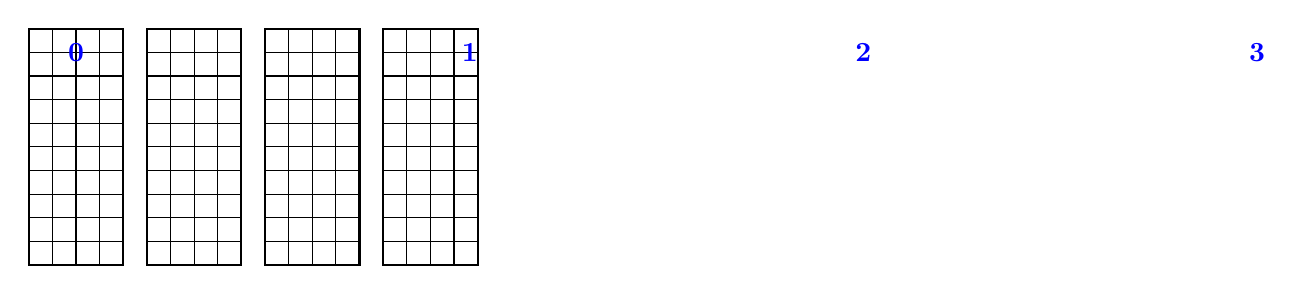
\begin{tikzpicture}[scale=0.3]
    % Grid for partition 0
    \draw[step=1, thin, black] (0,0) grid (4,10);
    \draw[thick] (0,0) rectangle (4,10);
    
    % Grid for partition 1
    \draw[step=1, thin, black, xshift=5cm] (0,0) grid (4,10);
    \draw[thick, xshift=5cm] (0,0) rectangle (4,10);
    
    % Grid for partition 2
    \draw[step=1, thin, black, xshift=10cm] (0,0) grid (4,10);
    \draw[thick, xshift=10cm] (0,0) rectangle (4,10);
    
    % Grid for partition 3
    \draw[step=1, thin, black, xshift=15cm] (0,0) grid (4,10);
    \draw[thick, xshift=15cm] (0,0) rectangle (4,10);

    % Partition labels
    \node[font=\bfseries, blue] at (2,9) {0};
    \node[font=\bfseries, blue, xshift=5cm] at (2,9) {1};
    \node[font=\bfseries, blue, xshift=10cm] at (2,9) {2};
    \node[font=\bfseries, blue, xshift=15cm] at (2,9) {3};
\end{tikzpicture}


% ======= split out
\begin{frame}\frametitle{M-to-N Restarts}
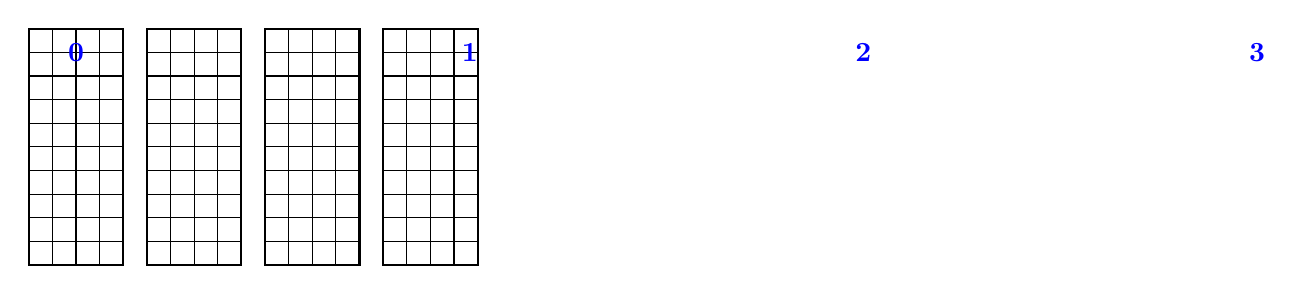
\begin{tikzpicture}[scale=0.3]
    % Grid for partition 0
    \draw[step=1, thin, black] (0,0) grid (4,10);
    \draw[thick] (0,0) rectangle (4,10);
    
    % Grid for partition 1
    \draw[step=1, thin, black, xshift=5cm] (0,0) grid (4,10);
    \draw[thick, xshift=5cm] (0,0) rectangle (4,10);
    
    % Grid for partition 2
    \draw[step=1, thin, black, xshift=10cm] (0,0) grid (4,10);
    \draw[thick, xshift=10cm] (0,0) rectangle (4,10);
    
    % Grid for partition 3
    \draw[step=1, thin, black, xshift=15cm] (0,0) grid (4,10);
    \draw[thick, xshift=15cm] (0,0) rectangle (4,10);

    % Partition labels
    \node[font=\bfseries, blue] at (2,9) {0};
    \node[font=\bfseries, blue, xshift=5cm] at (2,9) {1};
    \node[font=\bfseries, blue, xshift=10cm] at (2,9) {2};
    \node[font=\bfseries, blue, xshift=15cm] at (2,9) {3};
\end{tikzpicture}
\end{frame}

\begin{frame}\frametitle{M-to-N Restarts}
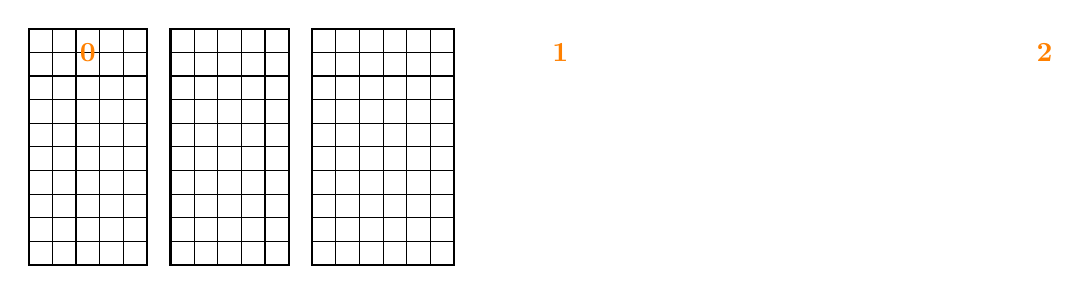
\begin{tikzpicture}[scale=0.3]
    % Grid for partition 0
    \draw[step=1, thin, black] (0,0) grid (5,10);
    \draw[thick] (0,0) rectangle (5,10);
    
    % Grid for partition 1
    \draw[step=1, thin, black, xshift=6cm] (0,0) grid (5,10);
    \draw[thick, xshift=6cm] (0,0) rectangle (5,10);
    
    % Grid for partition 2
    \draw[step=1, thin, black, xshift=12cm] (0,0) grid (6,10);
    \draw[thick, xshift=12cm] (0,0) rectangle (6,10);

    % Partition labels
    \node[font=\bfseries, orange] at (2.5,9) {0};
    \node[font=\bfseries, orange, xshift=6cm] at (2.5,9) {1};
    \node[font=\bfseries, orange, xshift=12cm] at (3,9) {2};
\end{tikzpicture}
\end{frame}
% =============

\begin{frame}
\frametitle{M-to-N Restart}
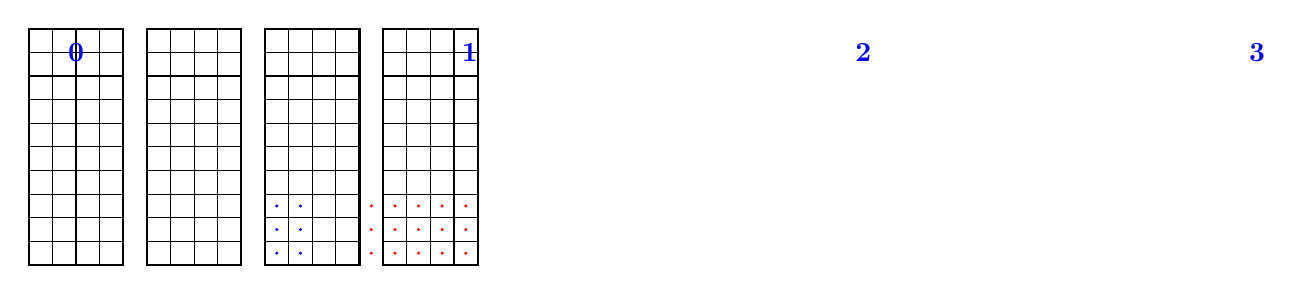
\begin{tikzpicture}[scale=0.3]
    % Grid for partition 0
    \draw[step=1, thin, black] (0,0) grid (4,10);
    \draw[thick] (0,0) rectangle (4,10);
    
    % Grid for partition 1
    \draw[step=1, thin, black, xshift=5cm] (0,0) grid (4,10);
    \draw[thick, xshift=5cm] (0,0) rectangle (4,10);
    
    % Grid for partition 2
    \draw[step=1, thin, black, xshift=10cm] (0,0) grid (4,10);
    \draw[thick, xshift=10cm] (0,0) rectangle (4,10);
    
    % Grid for partition 3
    \draw[step=1, thin, black, xshift=15cm] (0,0) grid (4,10);
    \draw[thick, xshift=15cm] (0,0) rectangle (4,10);

    % Red subregion
    \foreach \i in {11, 12, 13, 14, 15} {
        \foreach \j in {0, 1, 2} {
            \fill[red, xshift=15cm] (\i-12+0.5, \j+0.5) circle (2pt);
        }
    }
    
    % Blue subregion
    \foreach \i in {9, 10} {
        \foreach \j in {0, 1, 2} {
            \fill[blue, xshift=10cm] (\i-9+0.5, \j+0.5) circle (2pt);
        }
    }

    % Partition labels
    \node[font=\bfseries, blue] at (2,9) {0};
    \node[font=\bfseries, blue, xshift=5cm] at (2,9) {1};
    \node[font=\bfseries, blue, xshift=10cm] at (2,9) {2};
    \node[font=\bfseries, blue, xshift=15cm] at (2,9) {3};
\end{tikzpicture}
\end{frame}

\begin{frame}
\frametitle{M-to-N Restart}
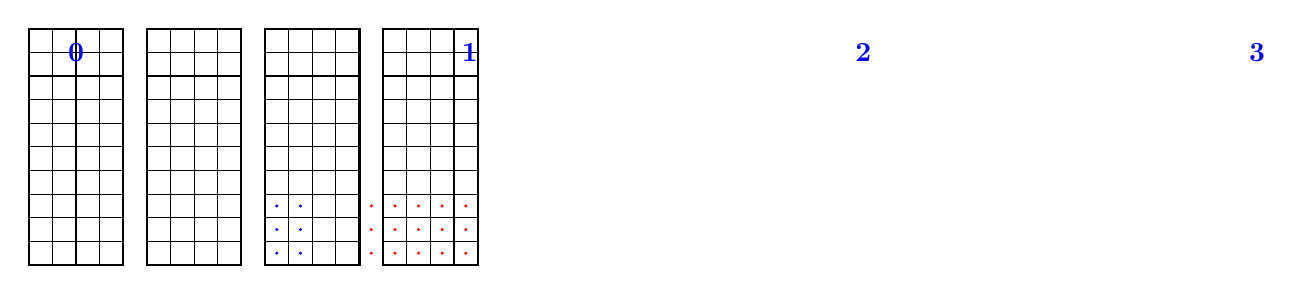
\begin{tikzpicture}[scale=0.3]
    % Grid for partition 0
    \draw[step=1, thin, black] (0,0) grid (4,10);
    \draw[thick] (0,0) rectangle (4,10);
    
    % Grid for partition 1
    \draw[step=1, thin, black, xshift=5cm] (0,0) grid (4,10);
    \draw[thick, xshift=5cm] (0,0) rectangle (4,10);
    
    % Grid for partition 2
    \draw[step=1, thin, black, xshift=10cm] (0,0) grid (4,10);
    \draw[thick, xshift=10cm] (0,0) rectangle (4,10);
    
    % Grid for partition 3
    \draw[step=1, thin, black, xshift=15cm] (0,0) grid (4,10);
    \draw[thick, xshift=15cm] (0,0) rectangle (4,10);
    
    % Red subregion
    \foreach \i in {11, 12, 13, 14, 15} {
        \foreach \j in {0, 1, 2} {
            \fill[red, xshift=15cm] (\i-12+0.5, \j+0.5) circle (2pt);
        }
    }
    
    % Blue subregion
    \foreach \i in {9, 10} {
        \foreach \j in {0, 1, 2} {
            \fill[blue, xshift=10cm] (\i-9+0.5, \j+0.5) circle (2pt);
        }
    }

    % Partition labels
    \node[font=\bfseries, blue] at (2,9) {0};
    \node[font=\bfseries, blue, xshift=5cm] at (2,9) {1};
    \node[font=\bfseries, blue, xshift=10cm] at (2,9) {2};
    \node[font=\bfseries, blue, xshift=15cm] at (2,9) {3};
\end{tikzpicture}
\end{frame}

\begin{frame}
\frametitle{M-to-N Restart}
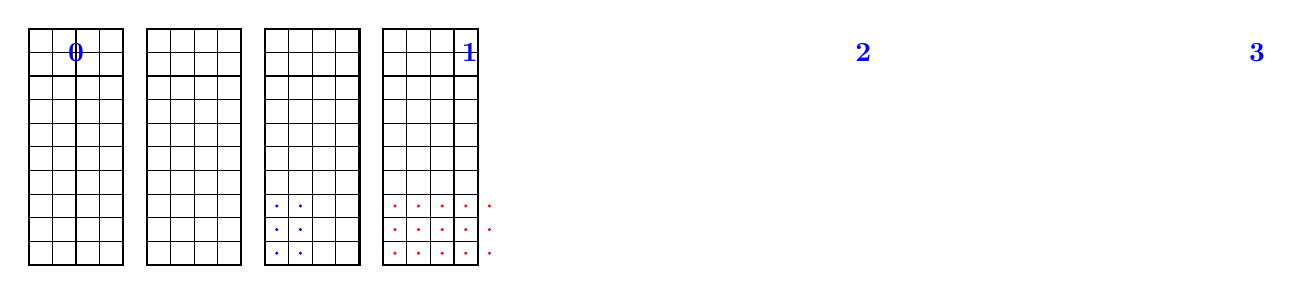
\begin{tikzpicture}[scale=0.3]
    % Grid for partition 0
    \draw[step=1, thin, black] (0,0) grid (4,10);
    \draw[thick] (0,0) rectangle (4,10);
    
    % Grid for partition 1
    \draw[step=1, thin, black, xshift=5cm] (0,0) grid (4,10);
    \draw[thick, xshift=5cm] (0,0) rectangle (4,10);
    
    % Grid for partition 2
    \draw[step=1, thin, black, xshift=10cm] (0,0) grid (4,10);
    \draw[thick, xshift=10cm] (0,0) rectangle (4,10);
    
    % Grid for partition 3
    \draw[step=1, thin, black, xshift=15cm] (0,0) grid (4,10);
    \draw[thick, xshift=15cm] (0,0) rectangle (4,10);
    
    % Red subregion in partition 3
    \foreach \i in {11, 12, 13, 14, 15} {
        \foreach \j in {0, 1, 2} {
            \fill[red, xshift=15cm] (\i-11+0.5, \j+0.5) circle (2pt);
        }
    }
    
    % Blue subregion in partition 2
    \foreach \i in {9, 10} {
        \foreach \j in {0, 1, 2} {
            \fill[blue, xshift=10cm] (\i-9+0.5, \j+0.5) circle (2pt);
        }
    }

    % Partition labels
    \node[font=\bfseries, blue] at (2,9) {0};
    \node[font=\bfseries, blue, xshift=5cm] at (2,9) {1};
    \node[font=\bfseries, blue, xshift=10cm] at (2,9) {2};
    \node[font=\bfseries, blue, xshift=15cm] at (2,9) {3};
\end{tikzpicture}
\end{frame}

\begin{frame}
\frametitle{M-to-N Restart}

% Partition 0
\begin{tikzpicture}[overlay, remember picture, shift={(2cm, 6cm)}]
    \draw[step=1, thin, black] (0,0) grid (4,10);
    \draw[thick] (0,0) rectangle (4,10);
    \node[font=\bfseries, blue] at (2,9) {0};
\end{tikzpicture}

% Partition 1 with blue subregion
\begin{tikzpicture}[overlay, remember picture, shift={(7cm, 6cm)}]
    \draw[step=1, thin, black] (0,0) grid (4,10);
    \draw[thick] (0,0) rectangle (4,10);
    \foreach \j in {0, 1, 2} {
        \fill[blue] (0.5, \j+0.5) circle (2pt);
        \fill[blue] (1.5, \j+0.5) circle (2pt);
    }
    \node[font=\bfseries, blue] at (2,9) {1};
\end{tikzpicture}

% Partition 2
\begin{tikzpicture}[overlay, remember picture, shift={(12cm, 6cm)}]
    \draw[step=1, thin, black] (0,0) grid (4,10);
    \draw[thick] (0,0) rectangle (4,10);
    \node[font=\bfseries, blue] at (2,9) {2};
\end{tikzpicture}

% Partition 3 with red subregion
\begin{tikzpicture}[overlay, remember picture, shift={(17cm, 6cm)}]
    \draw[step=1, thin, black] (0,0) grid (4,10);
    \draw[thick] (0,0) rectangle (4,10);
    \foreach \j in {0, 1, 2} {
        \fill[red] (0.5, \j+0.5) circle (2pt);
        \fill[red] (1.5, \j+0.5) circle (2pt);
        \fill[red] (2.5, \j+0.5) circle (2pt);
        \fill[red] (3.5, \j+0.5) circle (2pt);
    }
    \node[font=\bfseries, blue] at (2,9) {3};
\end{tikzpicture}

\end{frame}

\begin{frame}
\frametitle{M-to-N Restart}
\begin{tikzpicture}[scale=0.3, node distance=0.5cm]

    % Partition 0
    \node[draw, thick, minimum width=4cm, minimum height=10cm, inner sep=0pt, label={above:{\bfseries\color{blue}0}}] (part0) {};
    \draw[step=1, thin, black] (part0.south west) grid (part0.north east);
    
    % Partition 1 with blue subregion
    \node[draw, thick, minimum width=4cm, minimum height=10cm, inner sep=0pt, right=of part0, label={above:{\bfseries\color{blue}1}}] (part1) {};
    \draw[step=1, thin, black] (part1.south west) grid (part1.north east);
    \foreach \j in {0, 1, 2} {
        \fill[blue] ([xshift=0.5cm, yshift=(\j+0.5)*1cm]part1.south west) circle (2pt);
        \fill[blue] ([xshift=1.5cm, yshift=(\j+0.5)*1cm]part1.south west) circle (2pt);
    }
    
    % Partition 2
    \node[draw, thick, minimum width=4cm, minimum height=10cm, inner sep=0pt, right=of part1, label={above:{\bfseries\color{blue}2}}] (part2) {};
    \draw[step=1, thin, black] (part2.south west) grid (part2.north east);
    
    % Partition 3 with red subregion
    \node[draw, thick, minimum width=4cm, minimum height=10cm, inner sep=0pt, right=of part2, label={above:{\bfseries\color{blue}3}}] (part3) {};
    \draw[step=1, thin, black] (part3.south west) grid (part3.north east);
    \foreach \j in {0, 1, 2} {
        \fill[red] ([xshift=0.5cm, yshift=(\j+0.5)*1cm]part3.south west) circle (2pt);
        \fill[red] ([xshift=1.5cm, yshift=(\j+0.5)*1cm]part3.south west) circle (2pt);
        \fill[red] ([xshift=2.5cm, yshift=(\j+0.5)*1cm]part3.south west) circle (2pt);
        \fill[red] ([xshift=3.5cm, yshift=(\j+0.5)*1cm]part3.south west) circle (2pt);
    }
\end{tikzpicture}
\end{frame}

\begin{frame}
\frametitle{M-to-N Restart}
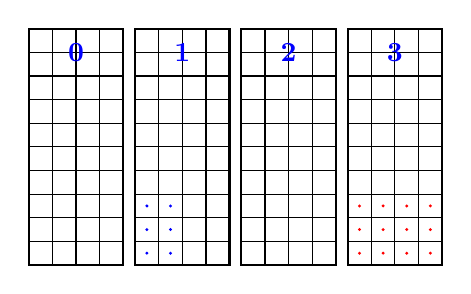
\begin{tikzpicture}[scale=0.3]

    % Partition 0
    \draw[step=1, thin, black] (0,0) grid (4,10);
    \draw[thick] (0,0) rectangle (4,10);
    \node[font=\bfseries, blue] at (2,9) {0};
    
    % Partition 1 with blue subregion
    \begin{scope}[xshift=4.5cm]
        \draw[step=1, thin, black] (0,0) grid (4,10);
        \draw[thick] (0,0) rectangle (4,10);
        \foreach \j in {0, 1, 2} {
            \fill[blue] (0.5, \j+0.5) circle (2pt);
            \fill[blue] (1.5, \j+0.5) circle (2pt);
        }
        \node[font=\bfseries, blue] at (2,9) {1};
    \end{scope}
    
    % Partition 2
    \begin{scope}[xshift=9cm]
        \draw[step=1, thin, black] (0,0) grid (4,10);
        \draw[thick] (0,0) rectangle (4,10);
        \node[font=\bfseries, blue] at (2,9) {2};
    \end{scope}
    
    % Partition 3 with red subregion
    \begin{scope}[xshift=13.5cm]
        \draw[step=1, thin, black] (0,0) grid (4,10);
        \draw[thick] (0,0) rectangle (4,10);
        \foreach \j in {0, 1, 2} {
            \fill[red] (0.5, \j+0.5) circle (2pt);
            \fill[red] (1.5, \j+0.5) circle (2pt);
            \fill[red] (2.5, \j+0.5) circle (2pt);
            \fill[red] (3.5, \j+0.5) circle (2pt);
        }
        \node[font=\bfseries, blue] at (2,9) {3};
    \end{scope}
\end{tikzpicture}
\end{frame}
\begin{frame}
\frametitle{M-to-N Restart}
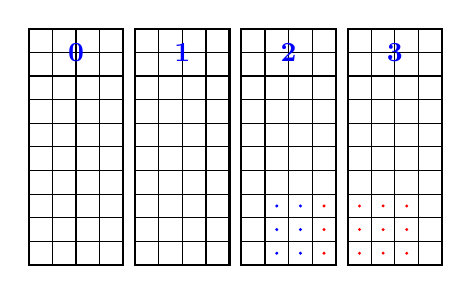
\begin{tikzpicture}[scale=0.3]

    % Partition 0
    \draw[step=1, thin, black] (0,0) grid (4,10);
    \draw[thick] (0,0) rectangle (4,10);
    \node[font=\bfseries, blue] at (2,9) {0};
    
    % Partition 1
    \begin{scope}[xshift=4.5cm]
        \draw[step=1, thin, black] (0,0) grid (4,10);
        \draw[thick] (0,0) rectangle (4,10);
        \node[font=\bfseries, blue] at (2,9) {1};
    \end{scope}
    
    % Partition 2 with blue and red subregions
    \begin{scope}[xshift=9cm]
        \draw[step=1, thin, black] (0,0) grid (4,10);
        \draw[thick] (0,0) rectangle (4,10);
        \foreach \j in {0, 1, 2} {
            \fill[blue] (1.5, \j+0.5) circle (2pt);
            \fill[blue] (2.5, \j+0.5) circle (2pt);
            \fill[red] (3.5, \j+0.5) circle (2pt);
        }
        \node[font=\bfseries, blue] at (2,9) {2};
    \end{scope}
    
    % Partition 3 with red subregion
    \begin{scope}[xshift=13.5cm]
        \draw[step=1, thin, black] (0,0) grid (4,10);
        \draw[thick] (0,0) rectangle (4,10);
        \foreach \j in {0, 1, 2} {
            \fill[red] (0.5, \j+0.5) circle (2pt);
            \fill[red] (1.5, \j+0.5) circle (2pt);
            \fill[red] (2.5, \j+0.5) circle (2pt);
        }
        \node[font=\bfseries, blue] at (2,9) {3};
    \end{scope}
\end{tikzpicture}
\end{frame}

\begin{frame}
\frametitle{M-to-N Restart}
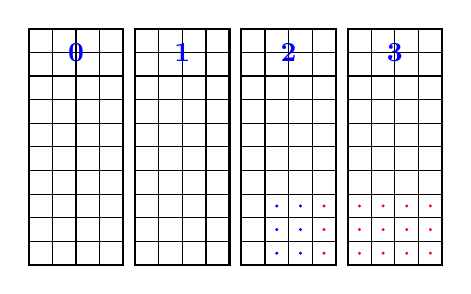
\begin{tikzpicture}[scale=0.3]

    % Partition 0
    \draw[step=1, thin, black] (0,0) grid (4,10);
    \draw[thick] (0,0) rectangle (4,10);
    \node[font=\bfseries, blue] at (2,9) {0};
    
    % Partition 1
    \begin{scope}[xshift=4.5cm]
        \draw[step=1, thin, black] (0,0) grid (4,10);
        \draw[thick] (0,0) rectangle (4,10);
        \node[font=\bfseries, blue] at (2,9) {1};
    \end{scope}
    
    % Partition 2 with blue and red subregions
    \begin{scope}[xshift=9cm]
        \draw[step=1, thin, black] (0,0) grid (4,10);
        \draw[thick] (0,0) rectangle (4,10);
        \foreach \j in {0, 1, 2} {
            \fill[blue] (1.5, \j+0.5) circle (2pt);
            \fill[blue] (2.5, \j+0.5) circle (2pt);
            \fill[red] (3.5, \j+0.5) circle (2pt);
        }
        \node[font=\bfseries, blue] at (2,9) {2};
    \end{scope}
    
    % Partition 3 with red subregion
    \begin{scope}[xshift=13.5cm]
        \draw[step=1, thin, black] (0,0) grid (4,10);
        \draw[thick] (0,0) rectangle (4,10);
        \foreach \j in {0, 1, 2} {
            \fill[red] (0.5, \j+0.5) circle (2pt);
            \fill[red] (1.5, \j+0.5) circle (2pt);
            \fill[red] (2.5, \j+0.5) circle (2pt);
            \fill[red] (3.5, \j+0.5) circle (2pt);  % added this line for the last column of red dots in partition 3
        }
        \node[font=\bfseries, blue] at (2,9) {3};
    \end{scope}
\end{tikzpicture}
\end{frame}
\begin{frame}
\frametitle{M-to-N Restart}
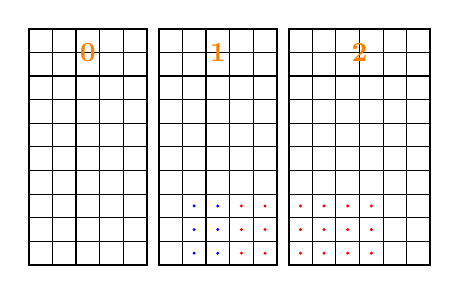
\begin{tikzpicture}[scale=0.3]

    % Partition 0
    \draw[step=1, thin, black] (0,0) grid (5,10);
    \draw[thick] (0,0) rectangle (5,10);
    \node[font=\bfseries, orange] at (2.5,9) {0};
    
    % Partition 1 with blue subregion
    \begin{scope}[xshift=5.5cm]
        \draw[step=1, thin, black] (0,0) grid (5,10);
        \draw[thick] (0,0) rectangle (5,10);
        \foreach \j in {0, 1, 2} {
            \fill[blue] (1.5, \j+0.5) circle (2pt);
            \fill[blue] (2.5, \j+0.5) circle (2pt);
            \fill[red] (3.5, \j+0.5) circle (2pt);
            \fill[red] (4.5, \j+0.5) circle (2pt);
        }
        \node[font=\bfseries, orange] at (2.5,9) {1};
    \end{scope}
    
    % Partition 2 with red subregion
    \begin{scope}[xshift=11cm]
        \draw[step=1, thin, black] (0,0) grid (6,10);
        \draw[thick] (0,0) rectangle (6,10);
        \foreach \j in {0, 1, 2} {
            \fill[red] (0.5, \j+0.5) circle (2pt);
            \fill[red] (1.5, \j+0.5) circle (2pt);
            \fill[red] (2.5, \j+0.5) circle (2pt);
            \fill[red] (3.5, \j+0.5) circle (2pt);
        }
        \node[font=\bfseries, orange] at (3,9) {2};
    \end{scope}
\end{tikzpicture}
\end{frame}

\begin{frame}
\frametitle{M-to-N Restart}
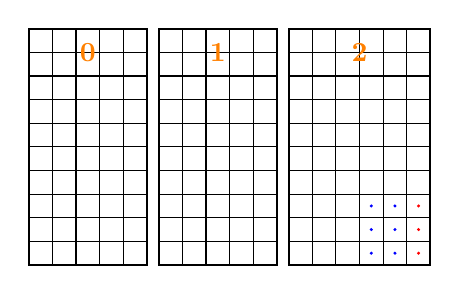
\begin{tikzpicture}[scale=0.3]

    % Partition 0
    \draw[step=1, thin, black] (0,0) grid (5,10);
    \draw[thick] (0,0) rectangle (5,10);
    \node[font=\bfseries, orange] at (2.5,9) {0};
    
    % Partition 1
    \begin{scope}[xshift=5.5cm]
        \draw[step=1, thin, black] (0,0) grid (5,10);
        \draw[thick] (0,0) rectangle (5,10);
        \node[font=\bfseries, orange] at (2.5,9) {1};
    \end{scope}
    
    % Partition 2 with blue and red subregions
    \begin{scope}[xshift=11cm]
        \draw[step=1, thin, black] (0,0) grid (6,10);
        \draw[thick] (0,0) rectangle (6,10);
        \foreach \j in {0, 1, 2} {
            \fill[blue] (3.5, \j+0.5) circle (2pt);  % shifted right by 2 columns
            \fill[blue] (4.5, \j+0.5) circle (2pt);  % shifted right by 2 columns
            \fill[red] (5.5, \j+0.5) circle (2pt);   % shifted right by 2 columns
        }
        \node[font=\bfseries, orange] at (3,9) {2};
    \end{scope}
\end{tikzpicture}
\end{frame}

\begin{frame}
\frametitle{M-to-N Restart}
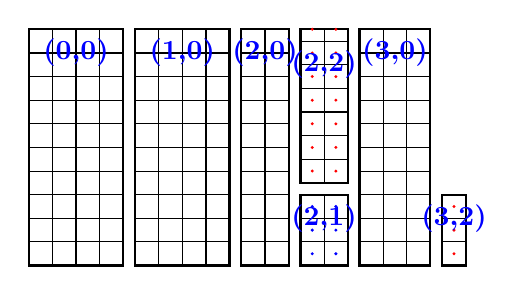
\begin{tikzpicture}[scale=0.3]

    % Partition (0,0)
    \draw[step=1, thin, black] (0,0) grid (4,10);
    \draw[thick] (0,0) rectangle (4,10);
    \node[font=\bfseries, blue] at (2,9) {(0,0)};

    % Partition (1,0)
    \begin{scope}[xshift=4.5cm]
        \draw[step=1, thin, black] (0,0) grid (4,10);
        \draw[thick] (0,0) rectangle (4,10);
        \node[font=\bfseries, blue] at (2,9) {(1,0)};
    \end{scope}

    % Partition (2,0)
    \begin{scope}[xshift=9cm]
        \draw[step=1, thin, black] (0,0) grid (2,10);
        \draw[thick] (0,0) rectangle (2,10);
        \node[font=\bfseries, blue] at (1,9) {(2,0)};
    \end{scope}

    % Partition (2,1) with blue subregion
    \begin{scope}[xshift=11.5cm]
        \draw[step=1, thin, black] (0,0) grid (2,3);
        \draw[thick] (0,0) rectangle (2,3);
        \foreach \j in {0, 1, 2} {
            \fill[blue] (0.5, \j+0.5) circle (2pt);
            \fill[blue] (1.5, \j+0.5) circle (2pt);
        }
        \node[font=\bfseries, blue] at (1,2) {(2,1)};
    \end{scope}

    % Partition (2,2) with red subregion
    \begin{scope}[xshift=11.5cm, yshift=3.5cm]
        \draw[step=1, thin, black] (0,0) grid (2,6.5);
        \draw[thick] (0,0) rectangle (2,6.5);
        \foreach \j in {0, 1, 2, 3, 4, 5, 6} {
            \fill[red] (0.5, \j+0.5) circle (2pt);
            \fill[red] (1.5, \j+0.5) circle (2pt);
        }
        \node[font=\bfseries, blue] at (1,5) {(2,2)};
    \end{scope}

    % Partition (3,0)
    \begin{scope}[xshift=14cm]
        \draw[step=1, thin, black] (0,0) grid (3,10);
        \draw[thick] (0,0) rectangle (3,10);
        \node[font=\bfseries, blue] at (1.5,9) {(3,0)};
    \end{scope}

    % Partition (3,2) with red subregion
    \begin{scope}[xshift=17.5cm]
        \draw[step=1, thin, black] (0,0) grid (1,3);
        \draw[thick] (0,0) rectangle (1,3);
        \foreach \j in {0, 1, 2} {
            \fill[red] (0.5, \j+0.5) circle (2pt);
        }
        \node[font=\bfseries, blue] at (0.5,2) {(3,2)};
    \end{scope}

\end{tikzpicture}
\end{frame}

\begin{frame}
\frametitle{Grid with Cutout}
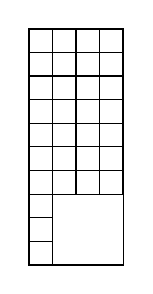
\begin{tikzpicture}[scale=0.3]

    % 4x10 grid
    \draw[step=1, thin, black] (0,0) grid (4,10);
    \draw[thick] (0,0) rectangle (4,10);
    
    % Cutout the 3x3 region in the lower right corner
    \fill[white, draw=black] (1,0) rectangle (4,3);

\end{tikzpicture}
\end{frame}

\begin{frame}
\frametitle{Grid with Adjusted Cutout}
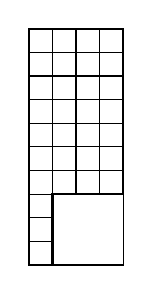
\begin{tikzpicture}[scale=0.3]

    % 4x10 grid
    \draw[step=1, thin, black] (0,0) grid (4,10);
    
    % Cutout the 3x3 region in the lower right corner
    \fill[white, draw=black] (1,0) rectangle (4,3);

    % Adjusted border
    \draw[thick] (0,0) -- (1,0) -- (1,3) -- (4,3) -- (4,10) -- (0,10) -- cycle;

\end{tikzpicture}
\end{frame}
\begin{frame}
\frametitle{Grid without Border on Cutout}
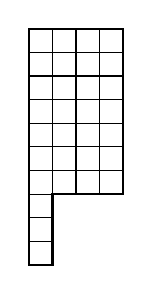
\begin{tikzpicture}[scale=0.3]

    % Draw only the visible cells
    \foreach \i in {0,1,2,3} {
        \foreach \j in {3,4,...,9} {
            \draw (\i,\j) rectangle (\i+1,\j+1);
        }
    }
    \draw (0,0) rectangle (1,3);
    \draw (0,0) rectangle (1,1);
    \draw (0,1) rectangle (1,2);
    \draw (0,2) rectangle (1,3);

    % Adjusted border
    \draw[thick] (0,0) -- (1,0) -- (1,3) -- (4,3) -- (4,10) -- (0,10) -- cycle;

\end{tikzpicture}
\end{frame}
\begin{frame}
\frametitle{M-to-N Restart}
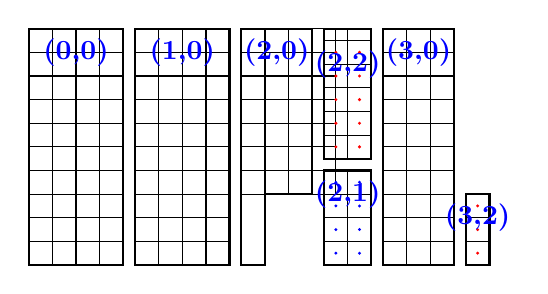
\begin{tikzpicture}[scale=0.3]

    % Partition (0,0)
    \draw[step=1, thin, black] (0,0) grid (4,10);
    \draw[thick] (0,0) rectangle (4,10);
    \node[font=\bfseries, blue] at (2,9) {(0,0)};

    % Partition (1,0)
    \begin{scope}[xshift=4.5cm]
        \draw[step=1, thin, black] (0,0) grid (4,10);
        \draw[thick] (0,0) rectangle (4,10);
        \node[font=\bfseries, blue] at (2,9) {(1,0)};
    \end{scope}

    % Partition (2,0) with adjusted cutout
    \begin{scope}[xshift=9cm]
        \foreach \i in {0,1,2,3} {
            \foreach \j in {3,4,...,9} {
                \draw (\i,\j) rectangle (\i+1,\j+1);
            }
        }
        \draw (0,0) rectangle (1,3);
        \draw[thick] (0,0) -- (1,0) -- (1,3) -- (3,3) -- (3,10) -- (0,10) -- cycle;
        \node[font=\bfseries, blue] at (1.5,9) {(2,0)};
    \end{scope}

    % Partition (2,1) with blue subregion
    \begin{scope}[xshift=12.5cm]
        \draw[step=1, thin, black] (0,0) grid (2,4);
        \draw[thick] (0,0) rectangle (2,4);
        \foreach \j in {0,1,2,3} {
            \fill[blue] (0.5, \j+0.5) circle (2pt);
            \fill[blue] (1.5, \j+0.5) circle (2pt);
        }
        \node[font=\bfseries, blue] at (1,3) {(2,1)};
    \end{scope}

    % Partition (2,2) with red subregion
    \begin{scope}[xshift=12.5cm, yshift=4.5cm]
        \draw[step=1, thin, black] (0,0) grid (2,5.5);
        \draw[thick] (0,0) rectangle (2,5.5);
        \foreach \j in {0,1,2,3,4} {
            \fill[red] (0.5, \j+0.5) circle (2pt);
            \fill[red] (1.5, \j+0.5) circle (2pt);
        }
        \node[font=\bfseries, blue] at (1,4) {(2,2)};
    \end{scope}

    % Partition (3,0)
    \begin{scope}[xshift=15cm]
        \draw[step=1, thin, black] (0,0) grid (3,10);
        \draw[thick] (0,0) rectangle (3,10);
        \node[font=\bfseries, blue] at (1.5,9) {(3,0)};
    \end{scope}

    % Partition (3,2) with red subregion
    \begin{scope}[xshift=18.5cm]
        \draw[step=1, thin, black] (0,0) grid (1,3);
        \draw[thick] (0,0) rectangle (1,3);
        \foreach \j in {0,1,2} {
            \fill[red] (0.5, \j+0.5) circle (2pt);
        }
        \node[font=\bfseries, blue] at (0.5,2) {(3,2)};
    \end{scope}

\end{tikzpicture}
\end{frame}

\begin{frame}
\frametitle{M-to-N Restart}
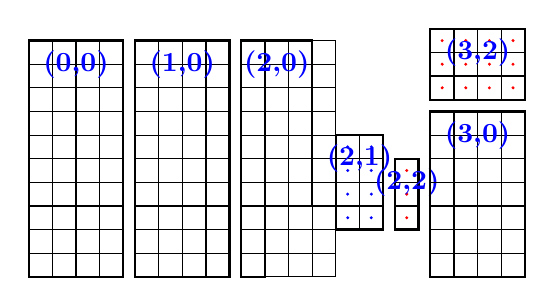
\begin{tikzpicture}[scale=0.3]

    % Partition (0,0)
    \draw[step=1, thin, black] (0,0) grid (4,10);
    \draw[thick] (0,0) rectangle (4,10);
    \node[font=\bfseries, blue] at (2,9) {(0,0)};

    % Partition (1,0)
    \begin{scope}[xshift=4.5cm]
        \draw[step=1, thin, black] (0,0) grid (4,10);
        \draw[thick] (0,0) rectangle (4,10);
        \node[font=\bfseries, blue] at (2,9) {(1,0)};
    \end{scope}

    % Partition (2,0) with corrected grid
    \begin{scope}[xshift=9cm]
        \foreach \i in {0,1,2,3} {
            \foreach \j in {0,1,2,3,4,...,9} {
                \draw (\i,\j) rectangle (\i+1,\j+1);
            }
        }
        \draw[thick] (0,0) -- (1,0) -- (1,3) -- (3,3) -- (3,10) -- (0,10) -- cycle;
        \node[font=\bfseries, blue] at (1.5,9) {(2,0)};
    \end{scope}

    % Partition (2,1) with blue subregion, adjusted position
    \begin{scope}[xshift=13cm, yshift=2cm]
        \draw[step=1, thin, black] (0,0) grid (2,4);
        \draw[thick] (0,0) rectangle (2,4);
        \foreach \j in {0,1,2,3} {
            \fill[blue] (0.5, \j+0.5) circle (2pt);
            \fill[blue] (1.5, \j+0.5) circle (2pt);
        }
        \node[font=\bfseries, blue] at (1,3) {(2,1)};
    \end{scope}

    % Partition (2,2) with red subregion, adjusted dimensions
    \begin{scope}[xshift=15.5cm, yshift=2cm]
        \draw[step=1, thin, black] (0,0) grid (1,3);
        \draw[thick] (0,0) rectangle (1,3);
        \foreach \j in {0,1,2} {
            \fill[red] (0.5, \j+0.5) circle (2pt);
        }
        \node[font=\bfseries, blue] at (0.5,2) {(2,2)};
    \end{scope}

    % Partition (3,0), adjusted dimensions
    \begin{scope}[xshift=17cm]
        \draw[step=1, thin, black] (0,0) grid (4,7);
        \draw[thick] (0,0) rectangle (4,7);
        \node[font=\bfseries, blue] at (2,6) {(3,0)};
    \end{scope}

    % Partition (3,2) with red subregion, adjusted dimensions
    \begin{scope}[xshift=17cm, yshift=7.5cm]
        \draw[step=1, thin, black] (0,0) grid (4,3);
        \draw[thick] (0,0) rectangle (4,3);
        \foreach \j in {0,1,2} {
            \fill[red] (0.5, \j+0.5) circle (2pt);
            \fill[red] (1.5, \j+0.5) circle (2pt);
            \fill[red] (2.5, \j+0.5) circle (2pt);
            \fill[red] (3.5, \j+0.5) circle (2pt);
        }
        \node[font=\bfseries, blue] at (2,2) {(3,2)};
    \end{scope}

\end{tikzpicture}
\end{frame}

\begin{frame}
\frametitle{M-to-N Restart}
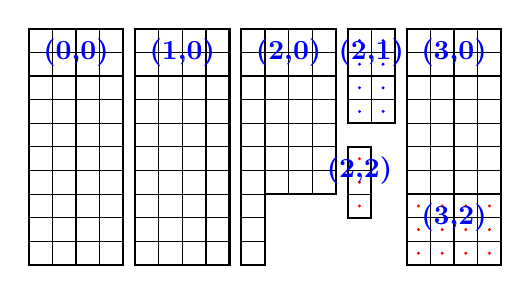
\begin{tikzpicture}[scale=0.3]

    % Partition (0,0)
    \draw[step=1, thin, black] (0,0) grid (4,10);
    \draw[thick] (0,0) rectangle (4,10);
    \node[font=\bfseries, blue] at (2,9) {(0,0)};

    % Partition (1,0)
    \begin{scope}[xshift=4.5cm]
        \draw[step=1, thin, black] (0,0) grid (4,10);
        \draw[thick] (0,0) rectangle (4,10);
        \node[font=\bfseries, blue] at (2,9) {(1,0)};
    \end{scope}

    % Partition (2,0) with the correct shape and border
    \begin{scope}[xshift=9cm]
        \foreach \i in {0,1,2,3} {
            \foreach \j in {3,4,...,9} {
                \draw (\i,\j) rectangle (\i+1,\j+1);
            }
        }
        \draw (0,0) rectangle (1,3);
        \draw (0,0) rectangle (1,1);
        \draw (0,1) rectangle (1,2);
        \draw (0,2) rectangle (1,3);
        \draw[thick] (0,0) -- (1,0) -- (1,3) -- (4,3) -- (4,10) -- (0,10) -- cycle;
        \node[font=\bfseries, blue] at (2,9) {(2,0)};
    \end{scope}

    % Partition (2,1) with blue subregion, adjusted position
    \begin{scope}[xshift=13.5cm, yshift=6cm]
        \draw[step=1, thin, black] (0,0) grid (2,4);
        \draw[thick] (0,0) rectangle (2,4);
        \foreach \j in {0,1,2,3} {
            \fill[blue] (0.5, \j+0.5) circle (2pt);
            \fill[blue] (1.5, \j+0.5) circle (2pt);
        }
        \node[font=\bfseries, blue] at (1,3) {(2,1)};
    \end{scope}

    % Partition (2,2) with red subregion, adjusted position
    \begin{scope}[xshift=13.5cm, yshift=2cm]
        \draw[step=1, thin, black] (0,0) grid (1,3);
        \draw[thick] (0,0) rectangle (1,3);
        \foreach \j in {0,1,2} {
            \fill[red] (0.5, \j+0.5) circle (2pt);
        }
        \node[font=\bfseries, blue] at (0.5,2) {(2,2)};
    \end{scope}

    % Partition (3,0), adjusted position and dimensions
    \begin{scope}[xshift=16cm, yshift=3cm]
        \draw[step=1, thin, black] (0,0) grid (4,7);
        \draw[thick] (0,0) rectangle (4,7);
        \node[font=\bfseries, blue] at (2,6) {(3,0)};
    \end{scope}

    % Partition (3,2) with red subregion, adjusted position
    \begin{scope}[xshift=16cm]
        \draw[step=1, thin, black] (0,0) grid (4,3);
        \draw[thick] (0,0) rectangle (4,3);
        \foreach \j in {0,1,2} {
            \fill[red] (0.5, \j+0.5) circle (2pt);
            \fill[red] (1.5, \j+0.5) circle (2pt);
            \fill[red] (2.5, \j+0.5) circle (2pt);
            \fill[red] (3.5, \j+0.5) circle (2pt);
        }
        \node[font=\bfseries, blue] at (2,2) {(3,2)};
    \end{scope}

\end{tikzpicture}
\end{frame}

\begin{frame}
\frametitle{M-to-N Restart}
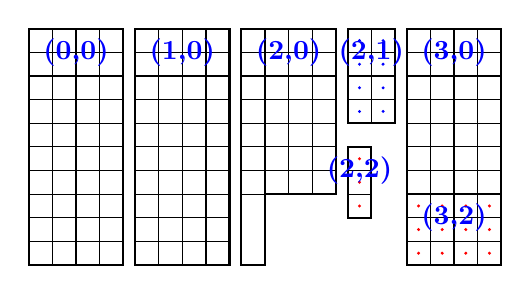
\begin{tikzpicture}[scale=0.3]

    % Partition (0,0)
    \draw[step=1, thin, black] (0,0) grid (4,10);
    \draw[thick] (0,0) rectangle (4,10);
    \node[font=\bfseries, blue] at (2,9) {(0,0)};

    % Partition (1,0)
    \begin{scope}[xshift=4.5cm]
        \draw[step=1, thin, black] (0,0) grid (4,10);
        \draw[thick] (0,0) rectangle (4,10);
        \node[font=\bfseries, blue] at (2,9) {(1,0)};
    \end{scope}

    % Partition (2,0) with the correct shape and border
    \begin{scope}[xshift=9cm]
        \foreach \i in {0,1,2,3} {
            \foreach \j in {3,4,...,9} {
                \draw (\i,\j) rectangle (\i+1,\j+1);
            }
        }
        \draw (0,0) rectangle (1,3);
        \draw[thick] (0,0) -- (1,0) -- (1,3) -- (4,3) -- (4,10) -- (0,10) -- cycle;
        \node[font=\bfseries, blue] at (2,9) {(2,0)};
    \end{scope}

    % Partition (2,1) with blue subregion, adjusted position
    \begin{scope}[xshift=13.5cm, yshift=6cm]
        \draw[step=1, thin, black] (0,0) grid (2,4);
        \draw[thick] (0,0) rectangle (2,4);
        \foreach \j in {0,1,2,3} {
            \fill[blue] (0.5, \j+0.5) circle (2pt);
            \fill[blue] (1.5, \j+0.5) circle (2pt);
        }
        \node[font=\bfseries, blue] at (1,3) {(2,1)};
    \end{scope}

    % Partition (2,2) with red subregion, adjusted position
    \begin{scope}[xshift=13.5cm, yshift=2cm]
        \draw[step=1, thin, black] (0,0) grid (1,3);
        \draw[thick] (0,0) rectangle (1,3);
        \foreach \j in {0,1,2} {
            \fill[red] (0.5, \j+0.5) circle (2pt);
        }
        \node[font=\bfseries, blue] at (0.5,2) {(2,2)};
    \end{scope}

    % Partition (3,0), adjusted position and dimensions
    \begin{scope}[xshift=16cm, yshift=3cm]
        \draw[step=1, thin, black] (0,0) grid (4,7);
        \draw[thick] (0,0) rectangle (4,7);
        \node[font=\bfseries, blue] at (2,6) {(3,0)};
    \end{scope}

    % Partition (3,2) with red subregion, adjusted position
    \begin{scope}[xshift=16cm]
        \draw[step=1, thin, black] (0,0) grid (4,3);
        \draw[thick] (0,0) rectangle (4,3);
        \foreach \j in {0,1,2} {
            \fill[red] (0.5, \j+0.5) circle (2pt);
            \fill[red] (1.5, \j+0.5) circle (2pt);
            \fill[red] (2.5, \j+0.5) circle (2pt);
            \fill[red] (3.5, \j+0.5) circle (2pt);
        }
        \node[font=\bfseries, blue] at (2,2) {(3,2)};
    \end{scope}

\end{tikzpicture}
\end{frame}

\begin{frame}
\frametitle{M-to-N Restart}
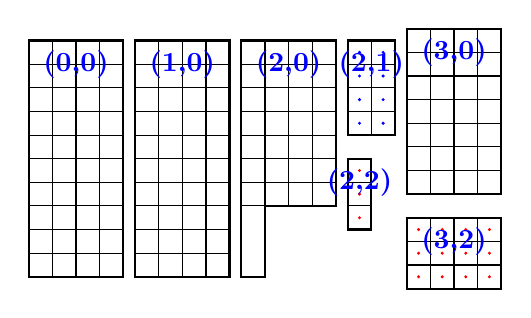
\begin{tikzpicture}[scale=0.3]

    % Partition (0,0)
    \draw[step=1, thin, black] (0,0) grid (4,10);
    \draw[thick] (0,0) rectangle (4,10);
    \node[font=\bfseries, blue] at (2,9) {(0,0)};

    % Partition (1,0)
    \begin{scope}[xshift=4.5cm]
        \draw[step=1, thin, black] (0,0) grid (4,10);
        \draw[thick] (0,0) rectangle (4,10);
        \node[font=\bfseries, blue] at (2,9) {(1,0)};
    \end{scope}

    % Partition (2,0) with the correct shape and border
    \begin{scope}[xshift=9cm]
        \foreach \i in {0,1,2,3} {
            \foreach \j in {3,4,...,9} {
                \draw (\i,\j) rectangle (\i+1,\j+1);
            }
        }
        \draw[thick] (0,0) -- (1,0) -- (1,3) -- (4,3) -- (4,10) -- (0,10) -- cycle;
        \node[font=\bfseries, blue] at (2,9) {(2,0)};
    \end{scope}

    % Partition (2,1) with blue subregion, adjusted position
    \begin{scope}[xshift=13.5cm, yshift=6cm]
        \draw[step=1, thin, black] (0,0) grid (2,4);
        \draw[thick] (0,0) rectangle (2,4);
        \foreach \j in {0,1,2,3} {
            \fill[blue] (0.5, \j+0.5) circle (2pt);
            \fill[blue] (1.5, \j+0.5) circle (2pt);
        }
        \node[font=\bfseries, blue] at (1,3) {(2,1)};
    \end{scope}

    % Partition (2,2) with red subregion, adjusted position
    \begin{scope}[xshift=13.5cm, yshift=2cm]
        \draw[step=1, thin, black] (0,0) grid (1,3);
        \draw[thick] (0,0) rectangle (1,3);
        \foreach \j in {0,1,2} {
            \fill[red] (0.5, \j+0.5) circle (2pt);
        }
        \node[font=\bfseries, blue] at (0.5,2) {(2,2)};
    \end{scope}

    % Partition (3,0), adjusted position and dimensions
    \begin{scope}[xshift=16cm, yshift=3.5cm]
        \draw[step=1, thin, black] (0,0) grid (4,7);
        \draw[thick] (0,0) rectangle (4,7);
        \node[font=\bfseries, blue] at (2,6) {(3,0)};
    \end{scope}

    % Partition (3,2) with red subregion, adjusted position
    \begin{scope}[xshift=16cm, yshift=-0.5cm]
        \draw[step=1, thin, black] (0,0) grid (4,3);
        \draw[thick] (0,0) rectangle (4,3);
        \foreach \j in {0,1,2} {
            \fill[red] (0.5, \j+0.5) circle (2pt);
            \fill[red] (1.5, \j+0.5) circle (2pt);
            \fill[red] (2.5, \j+0.5) circle (2pt);
            \fill[red] (3.5, \j+0.5) circle (2pt);
        }
        \node[font=\bfseries, blue] at (2,2) {(3,2)};
    \end{scope}

\end{tikzpicture}
\end{frame}


\begin{frame}
\frametitle{M-to-N Restart}
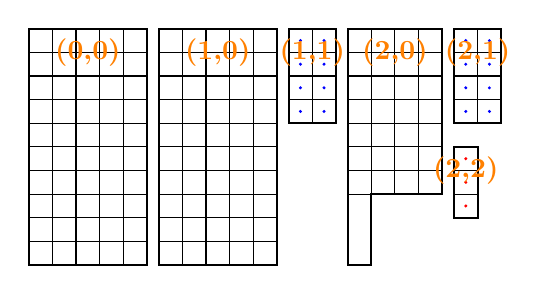
\begin{tikzpicture}[scale=0.3]

    % Partition (0,0)
    \draw[step=1, thin, black] (0,0) grid (5,10);
    \draw[thick] (0,0) rectangle (5,10);
    \node[font=\bfseries, orange] at (2.5,9) {(0,0)};

    % Partition (1,0)
    \begin{scope}[xshift=5.5cm]
        \draw[step=1, thin, black] (0,0) grid (5,10);
        \draw[thick] (0,0) rectangle (5,10);
        \node[font=\bfseries, orange] at (2.5,9) {(1,0)};
    \end{scope}

    % Partition (1,1) with blue subregion
    \begin{scope}[xshift=11cm, yshift=6cm]
        \draw[step=1, thin, black] (0,0) grid (2,4);
        \draw[thick] (0,0) rectangle (2,4);
        \foreach \j in {0,1,2,3} {
            \fill[blue] (0.5, \j+0.5) circle (2pt);
            \fill[blue] (1.5, \j+0.5) circle (2pt);
        }
        \node[font=\bfseries, orange] at (1,3) {(1,1)};
    \end{scope}

    % Partition (2,0) with the correct shape and border
    \begin{scope}[xshift=13.5cm]
        \foreach \i in {0,1,2,3} {
            \foreach \j in {3,4,...,9} {
                \draw (\i,\j) rectangle (\i+1,\j+1);
            }
        }
        \draw (0,0) rectangle (1,3);
        \draw[thick] (0,0) -- (1,0) -- (1,3) -- (4,3) -- (4,10) -- (0,10) -- cycle;
        \node[font=\bfseries, orange] at (2,9) {(2,0)};
    \end{scope}

    % Partition (2,1) with blue subregion, adjusted position
    \begin{scope}[xshift=18cm, yshift=6cm]
        \draw[step=1, thin, black] (0,0) grid (2,4);
        \draw[thick] (0,0) rectangle (2,4);
        \foreach \j in {0,1,2,3} {
            \fill[blue] (0.5, \j+0.5) circle (2pt);
            \fill[blue] (1.5, \j+0.5) circle (2pt);
        }
        \node[font=\bfseries, orange] at (1,3) {(2,1)};
    \end{scope}

    % Partition (2,2) with red subregion, adjusted position
    \begin{scope}[xshift=18cm, yshift=2cm]
        \draw[step=1, thin, black] (0,0) grid (1,3);
        \draw[thick] (0,0) rectangle (1,3);
        \foreach \j in {0,1,2} {
            \fill[red] (0.5, \j+0.5) circle (2pt);
        }
        \node[font=\bfseries, orange] at (0.5,2) {(2,2)};
    \end{scope}

\end{tikzpicture}
\end{frame}


\begin{frame}
\frametitle{M-to-N Restart}
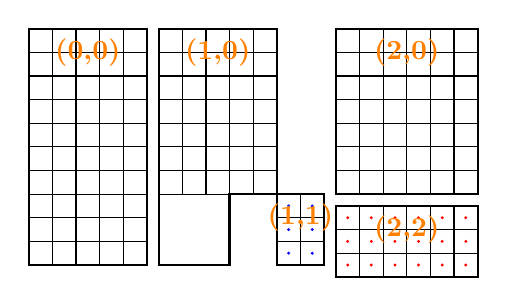
\begin{tikzpicture}[scale=0.3]

    % Partition (0,0)
    \draw[step=1, thin, black] (0,0) grid (5,10);
    \draw[thick] (0,0) rectangle (5,10);
    \node[font=\bfseries, orange] at (2.5,9) {(0,0)};

    % Partition (1,0) with the correct shape and border
    \begin{scope}[xshift=5.5cm]
        \foreach \i in {0,1,2,3,4} {
            \foreach \j in {3,4,...,9} {
                \draw (\i,\j) rectangle (\i+1,\j+1);
            }
        }
        \draw (0,0) rectangle (3,3);
        \draw[thick] (0,0) -- (3,0) -- (3,3) -- (5,3) -- (5,10) -- (0,10) -- cycle;
        \node[font=\bfseries, orange] at (2.5,9) {(1,0)};
    \end{scope}

    % Partition (1,1) with blue subregion
    \begin{scope}[xshift=10.5cm, yshift=0cm]
        \draw[step=1, thin, black] (0,0) grid (2,3);
        \draw[thick] (0,0) rectangle (2,3);
        \foreach \j in {0,1,2} {
            \fill[blue] (0.5, \j+0.5) circle (2pt);
            \fill[blue] (1.5, \j+0.5) circle (2pt);
        }
        \node[font=\bfseries, orange] at (1,2) {(1,1)};
    \end{scope}

    % Partition (2,0)
    \begin{scope}[xshift=13cm, yshift=3cm]
        \draw[step=1, thin, black] (0,0) grid (6,7);
        \draw[thick] (0,0) rectangle (6,7);
        \node[font=\bfseries, orange] at (3,6) {(2,0)};
    \end{scope}

    % Partition (2,2) with red subregion
    \begin{scope}[xshift=13cm, yshift=-0.5cm]
        \draw[step=1, thin, black] (0,0) grid (6,3);
        \draw[thick] (0,0) rectangle (6,3);
        \foreach \j in {0,1,2} {
            \fill[red] (0.5, \j+0.5) circle (2pt);
            \fill[red] (1.5, \j+0.5) circle (2pt);
            \fill[red] (2.5, \j+0.5) circle (2pt);
            \fill[red] (3.5, \j+0.5) circle (2pt);
            \fill[red] (4.5, \j+0.5) circle (2pt);
            \fill[red] (5.5, \j+0.5) circle (2pt);
        }
        \node[font=\bfseries, orange] at (3,2) {(2,2)};
    \end{scope}

\end{tikzpicture}
\end{frame}


\begin{frame}
\frametitle{M-to-N Restart}
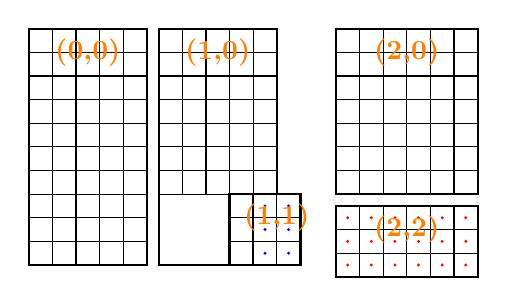
\begin{tikzpicture}[scale=0.3]

    % Partition (0,0)
    \draw[step=1, thin, black] (0,0) grid (5,10);
    \draw[thick] (0,0) rectangle (5,10);
    \node[font=\bfseries, orange] at (2.5,9) {(0,0)};

    % Partition (1,0) with the correct shape and border
    \begin{scope}[xshift=5.5cm]
        \foreach \i in {0,1,2,3,4} {
            \foreach \j in {3,4,...,9} {
                \draw (\i,\j) rectangle (\i+1,\j+1);
            }
        }
        \foreach \i in {3,4} {
            \foreach \j in {0,1,2} {
                \draw (\i,\j) rectangle (\i+1,\j+1);
            }
        }
        \draw[thick] (0,0) -- (3,0) -- (3,3) -- (5,3) -- (5,10) -- (0,10) -- cycle;
        \node[font=\bfseries, orange] at (2.5,9) {(1,0)};
    \end{scope}

    % Partition (1,1) with blue subregion, adjusted position
    \begin{scope}[xshift=9.5cm, yshift=0cm]
        \draw[step=1, thin, black] (0,0) grid (2,3);
        \draw[thick] (0,0) rectangle (2,3);
        \foreach \j in {0,1,2} {
            \fill[blue] (0.5, \j+0.5) circle (2pt);
            \fill[blue] (1.5, \j+0.5) circle (2pt);
        }
        \node[font=\bfseries, orange] at (1,2) {(1,1)};
    \end{scope}

    % Partition (2,0)
    \begin{scope}[xshift=13cm, yshift=3cm]
        \draw[step=1, thin, black] (0,0) grid (6,7);
        \draw[thick] (0,0) rectangle (6,7);
        \node[font=\bfseries, orange] at (3,6) {(2,0)};
    \end{scope}

    % Partition (2,2) with red subregion
    \begin{scope}[xshift=13cm, yshift=-0.5cm]
        \draw[step=1, thin, black] (0,0) grid (6,3);
        \draw[thick] (0,0) rectangle (6,3);
        \foreach \j in {0,1,2} {
            \fill[red] (0.5, \j+0.5) circle (2pt);
            \fill[red] (1.5, \j+0.5) circle (2pt);
            \fill[red] (2.5, \j+0.5) circle (2pt);
            \fill[red] (3.5, \j+0.5) circle (2pt);
            \fill[red] (4.5, \j+0.5) circle (2pt);
            \fill[red] (5.5, \j+0.5) circle (2pt);
        }
        \node[font=\bfseries, orange] at (3,2) {(2,2)};
    \end{scope}

\end{tikzpicture}
\end{frame}


\begin{frame}
\frametitle{M-to-N Restart}
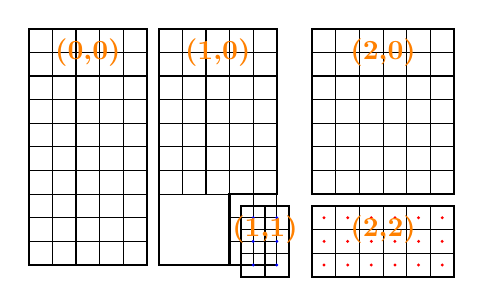
\begin{tikzpicture}[scale=0.3]

    % Partition (0,0)
    \draw[step=1, thin, black] (0,0) grid (5,10);
    \draw[thick] (0,0) rectangle (5,10);
    \node[font=\bfseries, orange] at (2.5,9) {(0,0)};

    % Partition (1,0) with the correct shape, border, and panhandle grid
    \begin{scope}[xshift=5.5cm]
        \foreach \i in {0,1,2,3,4} {
            \foreach \j in {3,4,...,9} {
                \draw (\i,\j) rectangle (\i+1,\j+1);
            }
        }
        \foreach \i in {3,4} {
            \foreach \j in {0,1,2} {
                \draw (\i,\j) rectangle (\i+1,\j+1);
            }
        }
        \draw[thick] (0,0) -- (3,0) -- (3,3) -- (5,3) -- (5,10) -- (0,10) -- cycle;
        \node[font=\bfseries, orange] at (2.5,9) {(1,0)};
    \end{scope}

    % Partition (1,1) with blue subregion, further adjusted position
    \begin{scope}[xshift=9cm, yshift=-0.5cm]
        \draw[step=1, thin, black] (0,0) grid (2,3);
        \draw[thick] (0,0) rectangle (2,3);
        \foreach \j in {0,1,2} {
            \fill[blue] (0.5, \j+0.5) circle (2pt);
            \fill[blue] (1.5, \j+0.5) circle (2pt);
        }
        \node[font=\bfseries, orange] at (1,2) {(1,1)};
    \end{scope}

    % Partition (2,0)
    \begin{scope}[xshift=12cm, yshift=3cm]
        \draw[step=1, thin, black] (0,0) grid (6,7);
        \draw[thick] (0,0) rectangle (6,7);
        \node[font=\bfseries, orange] at (3,6) {(2,0)};
    \end{scope}

    % Partition (2,2) with red subregion
    \begin{scope}[xshift=12cm, yshift=-0.5cm]
        \draw[step=1, thin, black] (0,0) grid (6,3);
        \draw[thick] (0,0) rectangle (6,3);
        \foreach \j in {0,1,2} {
            \fill[red] (0.5, \j+0.5) circle (2pt);
            \fill[red] (1.5, \j+0.5) circle (2pt);
            \fill[red] (2.5, \j+0.5) circle (2pt);
            \fill[red] (3.5, \j+0.5) circle (2pt);
            \fill[red] (4.5, \j+0.5) circle (2pt);
            \fill[red] (5.5, \j+0.5) circle (2pt);
        }
        \node[font=\bfseries, orange] at (3,2) {(2,2)};
    \end{scope}

\end{tikzpicture}
\end{frame}

\begin{frame}
\frametitle{M-to-N Restart}

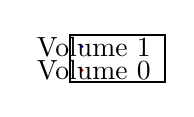
\begin{tikzpicture}[scale=0.3]
    % ... [rest of your existing TikZ picture]

    % Legend Box
    \begin{scope}[xshift=20cm, yshift=8cm]
        \draw[thick] (0,0) rectangle (4,-2); % The box around the legend
        \fill[blue] (0.5,-0.5) circle (2pt); % Blue dot
        \node[align=left] at (1,-0.5) {Volume 1};
        \fill[red] (0.5,-1.5) circle (2pt);  % Red dot
        \node[align=left] at (1,-1.5) {Volume 0};
    \end{scope}
\end{tikzpicture}

\end{frame}

\begin{frame}
\frametitle{M-to-N Restart}

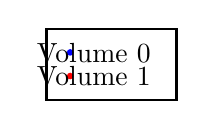
\begin{tikzpicture}[scale=0.3]
    % ... [rest of your existing TikZ picture]

    % Legend Box
    \begin{scope}[xshift=20cm, yshift=8cm]
        \draw[thick] (-0.5,0.5) rectangle (5,-2.5); % Adjusted the box around the legend
        \fill[blue] (0.5,-0.5) circle (4pt); % Bigger Blue dot
        \node[align=left] at (1.5,-0.5) {Volume 0};
        \fill[red] (0.5,-1.5) circle (4pt);  % Bigger Red dot
        \node[align=left] at (1.5,-1.5) {Volume 1};
    \end{scope}
\end{tikzpicture}

\end{frame}

\begin{frame}
\frametitle{M-to-N Restart}

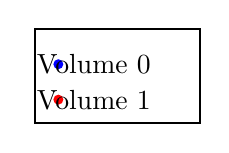
\begin{tikzpicture}[scale=0.3]
    % ... [rest of your existing TikZ picture]

    % Legend Box
    \begin{scope}[xshift=20cm, yshift=8cm]
        \draw[thick] (-1,1) rectangle (6,-3); % Adjusted the box to better fit around the legend
        
        \fill[blue] (0,-0.5) circle (6pt); % Larger Blue dot
        \node[align=left] at (1.5,-0.5) {Volume 0};
        
        \fill[red] (0,-2) circle (6pt);  % Larger Red dot
        \node[align=left] at (1.5,-2) {Volume 1};
    \end{scope}
\end{tikzpicture}

\end{frame}

\begin{frame}\frametitle{periodicity}
  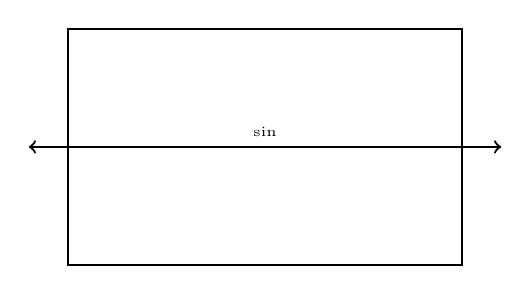
\begin{tikzpicture}
    % Draw a rectangle to represent the domain
    \draw[thick] (0,0) rectangle (5,3);
    
    % Periodicity on the left and right boundaries using double-headed arrow and sine wave
    \draw[<->, thick] (-0.5,1.5) -- node[sloped, above] {\tiny $\sin$} (5.5,1.5);
    
    % ... add other elements of your illustration
\end{tikzpicture}
\end{frame}

\begin{frame}\frametitle{periodicity}
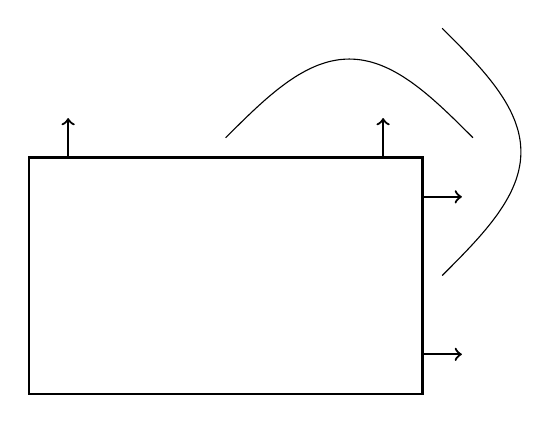
\begin{tikzpicture}
    % Draw a rectangle to represent the domain
    \draw[thick] (0,0) rectangle (5,3);
    
    % Block arrow with sine wave on the right boundary
    \draw[thick, ->] (5,0.5) -- (5.5,0.5);
    \draw[thick, ->] (5,2.5) -- (5.5,2.5);
    \draw[thick] (5,0.5) -- (5,2.5);
    \draw[domain=0:pi, smooth, variable=\y, shift={(5.25,1.5)}] plot ({sin(\y r)}, \y);

    % Block arrow with sine wave on the top boundary
    \draw[thick, ->] (0.5,3) -- (0.5,3.5);
    \draw[thick, ->] (4.5,3) -- (4.5,3.5);
    \draw[thick] (0.5,3) -- (4.5,3);
    \draw[domain=0:pi, smooth, variable=\x, shift={(2.5,3.25)}] plot (\x, {sin(\x r)});
    
    % ... add other elements of your illustration
\end{tikzpicture}
\end{frame}

    \node[anchor=south west, xshift=10pt, yshift=30pt] at (current page.south west) {
     
\includegraphics[width=0.07\textwidth]{github_logo.png}
    };

      % Text quadrant
  \begin{minipage}[t]{0.45\textwidth}
    \begin{itemize}
      \item Collected in short Lassen DAT on V100 GPUs
      \item Prediction domain and driver with increasing feature complexity
        \begin{itemize}
          \item Fluid: NS-only, 2 species
          \item AV: Fluid + Artificial Viscosity fields and eqns
          \item AVMix: AV + 7 species mixture EOS
          \item AVMixLimit: AVMix + species limiter
          \item FullPhysics: AVMixLimit + PowerLawTransport + Wall
        \end{itemize}
    \end{itemize}
  \end{minipage}
  \hfill
  % Top-right quadrant
  \begin{minipage}[t]{0.45\textwidth}
    \includegraphics[width=\linewidth]{/mnt/data/StartupTimes.pdf}
    \centering
    \small Startup Times
  \end{minipage}
  
  \vfill
  
  % Bottom-left quadrant
  \begin{minipage}[b]{0.45\textwidth}
    \includegraphics[width=\linewidth]{/mnt/data/RHSCompileTimes.pdf}
    \centering
    \small RHS Compile Times
  \end{minipage}
  \hfill
  % Bottom-right quadrant
  \begin{minipage}[b]{0.45\textwidth}
    \includegraphics[width=\linewidth]{/mnt/data/SimulationStepTimes.pdf}
    \centering
    \small Simulation Step Times
  \end{minipage}

    \begin{columns}[T]  % [T] is for top vertical alignment
    % Left Column
    \begin{column}{0.5\textwidth}
      % Top left: Text
      \begin{itemize}
        \item Collected in short Lassen DAT on V100 GPUs
        \item Prediction domain and driver with increasing feature complexity
          \begin{itemize}
            \item Fluid: NS-only, 2 species
            \item AV: Fluid + Artificial Viscosity fields and eqns
            \item AVMix: AV + 7 species mixture EOS
            \item AVMixLimit: AVMix + species limiter
            \item FullPhysics: AVMixLimit + PowerLawTransport + Wall
          \end{itemize}
      \end{itemize}
      % Bottom left: RHS Compile Times
      \includegraphics[width=\textwidth]{Figures/RHSCompileTimes.pdf}
    \end{column}
    
    % Right Column
    \begin{column}{0.5\textwidth}
      % Top right: Startup Times
      \includegraphics[width=\textwidth]{Figures/StartupTimes.pdf}
      % Bottom right: Simulation Step Times
      \includegraphics[width=\textwidth]{Figures/SimulationStepTimes.pdf}
    \end{column}
  \end{columns}
